%% CS 567 - 3D User Interfaces and Human-Centered Spatial AI - Fall 2026
%% Project Proposal.

\documentclass[sigconf,nonacm]{acmart}

\settopmatter{printacmref=false, printccs=false, printfolios=true}
\setcopyright{none}
\acmConference{CS 567: 3D User Interfaces and Human-Centered Spatial AI}{Fall 2026}{Colorado State University}

\usepackage{xcolor}
\usepackage{graphicx}

%% Gray italic instruction text. DELETE every \guide{...} before you submit.
\newcommand{\guide}[1]{{\color{gray}\itshape #1\par\medskip}}

\begin{document}

%% ---------------------------------------------------------------- title
\title{Physics You Can Feel: A Pseudo-Haptic VR Sandbox for Experiencing Mechanics and Material Properties}
\subtitle{CS567\_SVEN}

\author{Sven Skoglund}
\email{sven.skoglund@colostate.edu}
\affiliation{%
  \institution{Colorado State University}
  \department{Department of Computer Science}
  \city{Fort Collins}
  \state{CO}
  \country{USA}}

\renewcommand{\shortauthors}{CS567\_SVEN}

%% ---------------------------------------------------------------- abstract
%% NOTE(Sven): write the abstract LAST, then revise into your own voice. 100-150 words.
\begin{abstract}
Physical intuition about mass, volume, density, and friction, and about simple
machines such as levers and pulleys, is hard to build from equations and 2D
diagrams, and the demonstrations that would make it concrete are often
impractical or unsafe in a classroom. We propose an immersive virtual-reality
sandbox in which learners create, hold, weigh, and manipulate objects and simple
machines. Because commodity headsets cannot render true weight, we use
pseudo-haptic cues, modulating control-to-display gain and visual lag, so that a
heavier object feels heavier and a more heavily loaded lever feels harder to
move; the cue tracks mass and load, while density is revealed through the volume
of equal-mass blocks and through whether they float or sink. The application is
pure VR with no in-scene agent; agentic AI is instead the development workflow, an
AI coding agent that helps implement the Unity project. We evaluate the system
against closed-form physics and run a small within-subjects study testing whether
the weight cue improves how accurately learners predict outcomes that depend on
mass, density, and load.
\end{abstract}

\keywords{3D user interfaces; virtual reality; embodied learning; pseudo-haptics;
physics education; agentic AI; AI-assisted development}

\maketitle

%% ---------------------------------------------------------------- body
\section{Introduction and Motivation}
Introductory physics rests on relationships that students can state long before
they can predict with them. Density relates mass to volume, buoyancy determines
whether an object floats, friction resists sliding in proportion to the normal
load, and simple machines such as levers and pulleys trade force for distance.
The usual failure is not arithmetic but intuition. Asked whether a kilogram of
gold or a kilogram of ice is larger, which of two blocks slides farther down a
ramp, or where a load balances on a lever, many learners fall back on
misconceptions such as ``heavier means bigger.'' Textbooks and 2D simulations
show the formula and the result, yet they do not let a student \emph{feel} the
difference.

Doing the demonstration in real life is harder than it sounds: the comparisons
that isolate a single variable are exactly the ones that are awkward, expensive,
or unsafe to stage, since matched-mass materials are not classroom stock and
friction is hard to hold constant. Virtual reality can present these controlled
manipulations on demand, but a handheld controller weighs the same whatever it
represents, so the sensation many lessons depend on is missing. The open question
is whether a spatial interface can make physical properties and mechanical
behavior \emph{felt} well enough to matter, given that the dominant channel for
weight and force is the one current hardware cannot deliver.

%% Related Work lives in related-work.tex (expanded for Checkpoint 1).
%% ============================================================================
%% Related Work — Checkpoint 1 (expanded).
%%
%% Uses ten author-verified references in references.bib:
%%   slater2016enhancing, wu2020effectiveness, tsivitanidou2021inquiry,
%%   georgiou2021led, makransky2019gender, wang2019haptic, lecuyer2000pseudo,
%%   ujitoko2021pseudo, kim2022multisensory, bowman2004
%%
%% To use: %% ============================================================================
%% Related Work — Checkpoint 1 (expanded).
%%
%% Uses ten author-verified references in references.bib:
%%   slater2016enhancing, wu2020effectiveness, tsivitanidou2021inquiry,
%%   georgiou2021led, makransky2019gender, wang2019haptic, lecuyer2000pseudo,
%%   ujitoko2021pseudo, kim2022multisensory, bowman2004
%%
%% To use: %% ============================================================================
%% Related Work — Checkpoint 1 (expanded).
%%
%% Uses ten author-verified references in references.bib:
%%   slater2016enhancing, wu2020effectiveness, tsivitanidou2021inquiry,
%%   georgiou2021led, makransky2019gender, wang2019haptic, lecuyer2000pseudo,
%%   ujitoko2021pseudo, kim2022multisensory, bowman2004
%%
%% To use: \input{related-work} in main.tex in place of the current
%% \section{Related Work}.
%% ============================================================================

\section{Related Work}
Our sandbox sits at the intersection of four lines of research: immersive
virtual reality (VR) for science learning, the difficulty of rendering weight and
force on commodity hardware, the pseudo-haptic techniques that stand in for that
missing sensation, and the interaction-design foundations that make direct
manipulation legible. We review each in turn and close by stating what
distinguishes our approach.

\subsection{Immersive VR for Science Learning}
The pedagogical case for immersive VR rests less on visual fidelity than on the
sense of being present. Slater and S{\'a}nchez-Vives frame this through the place
illusion (the feeling of being in the virtual space) and the plausibility
illusion (the feeling that events are really happening), which together lead
users to respond to virtual events as if they were real~\cite{slater2016enhancing}.
For a physics sandbox this matters directly. If a learner treats a virtual block
and lever as real objects, then manipulating them can carry the intuitive weight
that a 2D simulation cannot.

Empirical work in physics education adds a consistent caveat: immersion helps,
but only when the learning experience is designed for it. A recent meta-analysis
by Wu et al.\ across many head-mounted display studies finds that immersive VR
yields a positive but moderate overall effect on learning performance, and that
this effect is strongly moderated by factors such as subject domain, learner
control, and how the experience is designed~\cite{wu2020effectiveness}.
Tsivitanidou, Georgiou, and Ioannou report on an inquiry-based immersive VR
physics activity from two angles: the learning experience they observe conceptual
gains alongside an interaction with learners' attitudinal
profiles~\cite{tsivitanidou2021inquiry}, and the design of that same experience,
which they document as a worked case of learning-experience
design~\cite{georgiou2021led}. We read this pair as evidence that immersive VR
physics learning is feasible and can produce conceptual gains; it establishes
that a VR physics activity can work, though it does not itself isolate felt weight
or the effect of a haptic cue. One common way to scaffold such experiences is an
embedded pedagogical agent. Makransky et al.\ studied one such agent and found a
gender-matching effect: a virtual instructor aided learning most when its
apparent gender matched the learner, a specific interaction rather than a general
endorsement of pedagogical agents~\cite{makransky2019gender}. Taken together,
these studies establish that immersive physics learning is promising but
design-sensitive. The value comes from what the learner is asked to do and how
the task is scaffolded, not from the headset itself. We take a deliberately
different scaffolding stance. Rather than an in-scene agent, we scaffold through
scene and task design, using tightly scoped scenarios that isolate a single
variable so that the cause of each outcome is unambiguous.

\subsection{The Missing Channel: Rendering Weight and Force}
The central obstacle for a physics-of-materials experience is that the very
quantity the lessons depend on, namely weight and the force needed to move a
loaded mechanism, is the one commodity that VR cannot deliver. A handheld
controller weighs the same whatever it represents. Wang et al.\ survey the state
of haptic display for VR and make clear that genuine, general-purpose force
feedback remains far from consumer reach, constrained by actuation, workspace,
and grounding requirements that headset-and-controller setups do not
meet~\cite{wang2019haptic}. Their survey frames the design problem for us
precisely. If we want a denser object to feel heavier on a Quest 2, we cannot
wait for the hardware to render the force, and must instead substitute perception
for physics.

\subsection{Pseudo-Haptics: Substituting Perception for Physics}
Pseudo-haptics addresses this gap by exploiting the dominance of vision over
proprioception. Manipulating the visual consequences of a motion, such as the
control-to-display gain or a small lag between hand and object, induces a felt
sense of weight, stiffness, or resistance without any force actuator. The
foundational demonstration comes from L{\'e}cuyer et al., who showed that
altering the visual response of an isometric input device makes users perceive
force and stiffness that no actuator produces, establishing that a
control-to-display manipulation alone can stand in for force
feedback~\cite{lecuyer2000pseudo}. Ujitoko and Ban survey the design space and
applications of pseudo-haptics, cataloguing how such visual manipulations
reliably produce haptic sensations and how they have been
applied~\cite{ujitoko2021pseudo}. Their taxonomy is the methodological backbone
for how we map mass and mechanical load onto gain and visual lag.

Two results ground our specific cue, the felt \emph{weight} of a held object.
Dominjon et al.\ manipulated the control/display ratio of a manipulated object in
a virtual environment and showed that this ratio directly changes its perceived
mass, so that the same physical motion can be made to feel heavier or lighter by
scaling its visual displacement~\cite{dominjon2005influence}. Rietzler et al.\
carried the same idea to consumer VR: by introducing perceivable offsets between
the tracked hand and the rendered object, they elicited a reliable sensation of
weight on a commodity headset with no force
hardware~\cite{rietzler2018breaking}. Together these establish that a gain or
tracking-offset manipulation can render felt weight on exactly the class of
device we target, and they fix the design variable for us: the cue must track an
object's \emph{mass}, the quantity that determines weight, rather than its
density. These techniques are not limited to lifting a single object. The same
principle of modulating the visual outcome of an effort extends naturally to the
resistance of operating a machine, such as a lever that grows harder to move as
its load increases.

\subsection{Foundations of 3D Interaction}
Whatever the illusion, the learner must first be able to reach out, grab, and
place objects fluidly, or the physics never gets probed. We ground our
interaction design in Bowman et al.'s canonical treatment of 3D user interfaces,
which formalizes selection, manipulation, and travel as the core tasks of spatial
interaction and catalogues the techniques for each~\cite{bowman2004}. This
foundation informs the grab-and-place model at the heart of the sandbox and keeps
our contribution, the pseudo-haptic property mapping, layered on top of
well-understood manipulation techniques rather than reinventing them.

\subsection{What Is Different About Our Approach}
Two gaps emerge from this literature. First, immersive physics studies
consistently deliver visual and interactive experiences but rarely give learners
a genuine felt contrast in weight between objects. A student may see that two
blocks differ, but does not feel one resist more than the other. Second,
pseudo-haptic studies convincingly render the felt weight of an isolated
object~\cite{dominjon2005influence, rietzler2018breaking}, but seldom span both
material properties (density, buoyancy, friction) and simple machines (levers,
pulleys) within one coherent environment and interaction model. Our sandbox
targets this intersection. We use pseudo-haptic gain and visual-lag modulation as
a unifying mechanism that makes an unrenderable physical quantity perceptible
across a family of controlled, single-variable scenarios, and we extend the same
mechanism from holding a heavier object to feeling a loaded lever push back.
Crucially, the cue tracks \emph{mass} for held objects and \emph{load} for the
lever, the quantities that actually determine weight and effort, so that density
is taught where it belongs, through the volume difference between equal-mass
blocks and through float-or-sink behavior, rather than being conflated with
heaviness. Because our contribution is an interaction technique for making a
physical quantity felt, we evaluate it at two levels: a system level, checking
that the cues behave monotonically with the underlying physics and that each
scenario matches its closed-form prediction; and a human level, a within-subjects
study testing whether the weight cue changes how accurately learners predict
outcomes that depend on mass, density, and load.
 in main.tex in place of the current
%% \section{Related Work}.
%% ============================================================================

\section{Related Work}
Our sandbox sits at the intersection of four lines of research: immersive
virtual reality (VR) for science learning, the difficulty of rendering weight and
force on commodity hardware, the pseudo-haptic techniques that stand in for that
missing sensation, and the interaction-design foundations that make direct
manipulation legible. We review each in turn and close by stating what
distinguishes our approach.

\subsection{Immersive VR for Science Learning}
The pedagogical case for immersive VR rests less on visual fidelity than on the
sense of being present. Slater and S{\'a}nchez-Vives frame this through the place
illusion (the feeling of being in the virtual space) and the plausibility
illusion (the feeling that events are really happening), which together lead
users to respond to virtual events as if they were real~\cite{slater2016enhancing}.
For a physics sandbox this matters directly. If a learner treats a virtual block
and lever as real objects, then manipulating them can carry the intuitive weight
that a 2D simulation cannot.

Empirical work in physics education adds a consistent caveat: immersion helps,
but only when the learning experience is designed for it. A recent meta-analysis
by Wu et al.\ across many head-mounted display studies finds that immersive VR
yields a positive but moderate overall effect on learning performance, and that
this effect is strongly moderated by factors such as subject domain, learner
control, and how the experience is designed~\cite{wu2020effectiveness}.
Tsivitanidou, Georgiou, and Ioannou report on an inquiry-based immersive VR
physics activity from two angles: the learning experience they observe conceptual
gains alongside an interaction with learners' attitudinal
profiles~\cite{tsivitanidou2021inquiry}, and the design of that same experience,
which they document as a worked case of learning-experience
design~\cite{georgiou2021led}. We read this pair as evidence that immersive VR
physics learning is feasible and can produce conceptual gains; it establishes
that a VR physics activity can work, though it does not itself isolate felt weight
or the effect of a haptic cue. One common way to scaffold such experiences is an
embedded pedagogical agent. Makransky et al.\ studied one such agent and found a
gender-matching effect: a virtual instructor aided learning most when its
apparent gender matched the learner, a specific interaction rather than a general
endorsement of pedagogical agents~\cite{makransky2019gender}. Taken together,
these studies establish that immersive physics learning is promising but
design-sensitive. The value comes from what the learner is asked to do and how
the task is scaffolded, not from the headset itself. We take a deliberately
different scaffolding stance. Rather than an in-scene agent, we scaffold through
scene and task design, using tightly scoped scenarios that isolate a single
variable so that the cause of each outcome is unambiguous.

\subsection{The Missing Channel: Rendering Weight and Force}
The central obstacle for a physics-of-materials experience is that the very
quantity the lessons depend on, namely weight and the force needed to move a
loaded mechanism, is the one commodity that VR cannot deliver. A handheld
controller weighs the same whatever it represents. Wang et al.\ survey the state
of haptic display for VR and make clear that genuine, general-purpose force
feedback remains far from consumer reach, constrained by actuation, workspace,
and grounding requirements that headset-and-controller setups do not
meet~\cite{wang2019haptic}. Their survey frames the design problem for us
precisely. If we want a denser object to feel heavier on a Quest 2, we cannot
wait for the hardware to render the force, and must instead substitute perception
for physics.

\subsection{Pseudo-Haptics: Substituting Perception for Physics}
Pseudo-haptics addresses this gap by exploiting the dominance of vision over
proprioception. Manipulating the visual consequences of a motion, such as the
control-to-display gain or a small lag between hand and object, induces a felt
sense of weight, stiffness, or resistance without any force actuator. The
foundational demonstration comes from L{\'e}cuyer et al., who showed that
altering the visual response of an isometric input device makes users perceive
force and stiffness that no actuator produces, establishing that a
control-to-display manipulation alone can stand in for force
feedback~\cite{lecuyer2000pseudo}. Ujitoko and Ban survey the design space and
applications of pseudo-haptics, cataloguing how such visual manipulations
reliably produce haptic sensations and how they have been
applied~\cite{ujitoko2021pseudo}. Their taxonomy is the methodological backbone
for how we map mass and mechanical load onto gain and visual lag.

Two results ground our specific cue, the felt \emph{weight} of a held object.
Dominjon et al.\ manipulated the control/display ratio of a manipulated object in
a virtual environment and showed that this ratio directly changes its perceived
mass, so that the same physical motion can be made to feel heavier or lighter by
scaling its visual displacement~\cite{dominjon2005influence}. Rietzler et al.\
carried the same idea to consumer VR: by introducing perceivable offsets between
the tracked hand and the rendered object, they elicited a reliable sensation of
weight on a commodity headset with no force
hardware~\cite{rietzler2018breaking}. Together these establish that a gain or
tracking-offset manipulation can render felt weight on exactly the class of
device we target, and they fix the design variable for us: the cue must track an
object's \emph{mass}, the quantity that determines weight, rather than its
density. These techniques are not limited to lifting a single object. The same
principle of modulating the visual outcome of an effort extends naturally to the
resistance of operating a machine, such as a lever that grows harder to move as
its load increases.

\subsection{Foundations of 3D Interaction}
Whatever the illusion, the learner must first be able to reach out, grab, and
place objects fluidly, or the physics never gets probed. We ground our
interaction design in Bowman et al.'s canonical treatment of 3D user interfaces,
which formalizes selection, manipulation, and travel as the core tasks of spatial
interaction and catalogues the techniques for each~\cite{bowman2004}. This
foundation informs the grab-and-place model at the heart of the sandbox and keeps
our contribution, the pseudo-haptic property mapping, layered on top of
well-understood manipulation techniques rather than reinventing them.

\subsection{What Is Different About Our Approach}
Two gaps emerge from this literature. First, immersive physics studies
consistently deliver visual and interactive experiences but rarely give learners
a genuine felt contrast in weight between objects. A student may see that two
blocks differ, but does not feel one resist more than the other. Second,
pseudo-haptic studies convincingly render the felt weight of an isolated
object~\cite{dominjon2005influence, rietzler2018breaking}, but seldom span both
material properties (density, buoyancy, friction) and simple machines (levers,
pulleys) within one coherent environment and interaction model. Our sandbox
targets this intersection. We use pseudo-haptic gain and visual-lag modulation as
a unifying mechanism that makes an unrenderable physical quantity perceptible
across a family of controlled, single-variable scenarios, and we extend the same
mechanism from holding a heavier object to feeling a loaded lever push back.
Crucially, the cue tracks \emph{mass} for held objects and \emph{load} for the
lever, the quantities that actually determine weight and effort, so that density
is taught where it belongs, through the volume difference between equal-mass
blocks and through float-or-sink behavior, rather than being conflated with
heaviness. Because our contribution is an interaction technique for making a
physical quantity felt, we evaluate it at two levels: a system level, checking
that the cues behave monotonically with the underlying physics and that each
scenario matches its closed-form prediction; and a human level, a within-subjects
study testing whether the weight cue changes how accurately learners predict
outcomes that depend on mass, density, and load.
 in main.tex in place of the current
%% \section{Related Work}.
%% ============================================================================

\section{Related Work}
Our sandbox sits at the intersection of four lines of research: immersive
virtual reality (VR) for science learning, the difficulty of rendering weight and
force on commodity hardware, the pseudo-haptic techniques that stand in for that
missing sensation, and the interaction-design foundations that make direct
manipulation legible. We review each in turn and close by stating what
distinguishes our approach.

\subsection{Immersive VR for Science Learning}
The pedagogical case for immersive VR rests less on visual fidelity than on the
sense of being present. Slater and S{\'a}nchez-Vives frame this through the place
illusion (the feeling of being in the virtual space) and the plausibility
illusion (the feeling that events are really happening), which together lead
users to respond to virtual events as if they were real~\cite{slater2016enhancing}.
For a physics sandbox this matters directly. If a learner treats a virtual block
and lever as real objects, then manipulating them can carry the intuitive weight
that a 2D simulation cannot.

Empirical work in physics education adds a consistent caveat: immersion helps,
but only when the learning experience is designed for it. A recent meta-analysis
by Wu et al.\ across many head-mounted display studies finds that immersive VR
yields a positive but moderate overall effect on learning performance, and that
this effect is strongly moderated by factors such as subject domain, learner
control, and how the experience is designed~\cite{wu2020effectiveness}.
Tsivitanidou, Georgiou, and Ioannou report on an inquiry-based immersive VR
physics activity from two angles: the learning experience they observe conceptual
gains alongside an interaction with learners' attitudinal
profiles~\cite{tsivitanidou2021inquiry}, and the design of that same experience,
which they document as a worked case of learning-experience
design~\cite{georgiou2021led}. We read this pair as evidence that immersive VR
physics learning is feasible and can produce conceptual gains; it establishes
that a VR physics activity can work, though it does not itself isolate felt weight
or the effect of a haptic cue. One common way to scaffold such experiences is an
embedded pedagogical agent. Makransky et al.\ studied one such agent and found a
gender-matching effect: a virtual instructor aided learning most when its
apparent gender matched the learner, a specific interaction rather than a general
endorsement of pedagogical agents~\cite{makransky2019gender}. Taken together,
these studies establish that immersive physics learning is promising but
design-sensitive. The value comes from what the learner is asked to do and how
the task is scaffolded, not from the headset itself. We take a deliberately
different scaffolding stance. Rather than an in-scene agent, we scaffold through
scene and task design, using tightly scoped scenarios that isolate a single
variable so that the cause of each outcome is unambiguous.

\subsection{The Missing Channel: Rendering Weight and Force}
The central obstacle for a physics-of-materials experience is that the very
quantity the lessons depend on, namely weight and the force needed to move a
loaded mechanism, is the one commodity that VR cannot deliver. A handheld
controller weighs the same whatever it represents. Wang et al.\ survey the state
of haptic display for VR and make clear that genuine, general-purpose force
feedback remains far from consumer reach, constrained by actuation, workspace,
and grounding requirements that headset-and-controller setups do not
meet~\cite{wang2019haptic}. Their survey frames the design problem for us
precisely. If we want a denser object to feel heavier on a Quest 2, we cannot
wait for the hardware to render the force, and must instead substitute perception
for physics.

\subsection{Pseudo-Haptics: Substituting Perception for Physics}
Pseudo-haptics addresses this gap by exploiting the dominance of vision over
proprioception. Manipulating the visual consequences of a motion, such as the
control-to-display gain or a small lag between hand and object, induces a felt
sense of weight, stiffness, or resistance without any force actuator. The
foundational demonstration comes from L{\'e}cuyer et al., who showed that
altering the visual response of an isometric input device makes users perceive
force and stiffness that no actuator produces, establishing that a
control-to-display manipulation alone can stand in for force
feedback~\cite{lecuyer2000pseudo}. Ujitoko and Ban survey the design space and
applications of pseudo-haptics, cataloguing how such visual manipulations
reliably produce haptic sensations and how they have been
applied~\cite{ujitoko2021pseudo}. Their taxonomy is the methodological backbone
for how we map mass and mechanical load onto gain and visual lag.

Two results ground our specific cue, the felt \emph{weight} of a held object.
Dominjon et al.\ manipulated the control/display ratio of a manipulated object in
a virtual environment and showed that this ratio directly changes its perceived
mass, so that the same physical motion can be made to feel heavier or lighter by
scaling its visual displacement~\cite{dominjon2005influence}. Rietzler et al.\
carried the same idea to consumer VR: by introducing perceivable offsets between
the tracked hand and the rendered object, they elicited a reliable sensation of
weight on a commodity headset with no force
hardware~\cite{rietzler2018breaking}. Together these establish that a gain or
tracking-offset manipulation can render felt weight on exactly the class of
device we target, and they fix the design variable for us: the cue must track an
object's \emph{mass}, the quantity that determines weight, rather than its
density. These techniques are not limited to lifting a single object. The same
principle of modulating the visual outcome of an effort extends naturally to the
resistance of operating a machine, such as a lever that grows harder to move as
its load increases.

\subsection{Foundations of 3D Interaction}
Whatever the illusion, the learner must first be able to reach out, grab, and
place objects fluidly, or the physics never gets probed. We ground our
interaction design in Bowman et al.'s canonical treatment of 3D user interfaces,
which formalizes selection, manipulation, and travel as the core tasks of spatial
interaction and catalogues the techniques for each~\cite{bowman2004}. This
foundation informs the grab-and-place model at the heart of the sandbox and keeps
our contribution, the pseudo-haptic property mapping, layered on top of
well-understood manipulation techniques rather than reinventing them.

\subsection{What Is Different About Our Approach}
Two gaps emerge from this literature. First, immersive physics studies
consistently deliver visual and interactive experiences but rarely give learners
a genuine felt contrast in weight between objects. A student may see that two
blocks differ, but does not feel one resist more than the other. Second,
pseudo-haptic studies convincingly render the felt weight of an isolated
object~\cite{dominjon2005influence, rietzler2018breaking}, but seldom span both
material properties (density, buoyancy, friction) and simple machines (levers,
pulleys) within one coherent environment and interaction model. Our sandbox
targets this intersection. We use pseudo-haptic gain and visual-lag modulation as
a unifying mechanism that makes an unrenderable physical quantity perceptible
across a family of controlled, single-variable scenarios, and we extend the same
mechanism from holding a heavier object to feeling a loaded lever push back.
Crucially, the cue tracks \emph{mass} for held objects and \emph{load} for the
lever, the quantities that actually determine weight and effort, so that density
is taught where it belongs, through the volume difference between equal-mass
blocks and through float-or-sink behavior, rather than being conflated with
heaviness. Because our contribution is an interaction technique for making a
physical quantity felt, we evaluate it at two levels: a system level, checking
that the cues behave monotonically with the underlying physics and that each
scenario matches its closed-form prediction; and a human level, a within-subjects
study testing whether the weight cue changes how accurately learners predict
outcomes that depend on mass, density, and load.


\section{Approach}
We will build a VR ``physics sandbox'' in which the learner constructs and probes
scenarios and the interface makes the governing quantity perceptible. Early
scenarios target material properties: pick up two blocks and feel which is
heavier on a balance, drop them in water to see buoyancy, and drag them across a
ramp to compare friction. Density is made visible rather than felt: two
\emph{equal-mass} blocks of different materials differ in size, so the denser one
is visibly smaller, and the same pair floats or sinks by density in the tank. The
same interaction model extends to mechanical devices, such as placing weights on
a lever to find its balance point or routing a rope through a pulley to feel the
reduced effort. In each case a single variable is isolated so the outcome has a
clear cause. Weight and resistance are conveyed through pseudo-haptics,
modulating control-to-display gain and visual lag so that a heavier block feels
heavier and a more heavily loaded lever feels harder to
move~\cite{ujitoko2021pseudo, dominjon2005influence, rietzler2018breaking}. The
cue tracks an object's \emph{mass}, the quantity that determines its weight,
rather than its density: equal-mass blocks weigh the same whatever their material,
so making a denser block feel heavier would teach the very ``heavier means
bigger'' misconception the sandbox sets out to correct. This is where the project
complies with HCI research in \textbf{Virtual Reality}: the contribution is an
interaction technique for making an unrenderable physical quantity perceptible
through direct, embodied manipulation.

The second aspect is the \textbf{agentic-AI} development workflow, and we are
deliberate about the distinction the assignment draws. The finished application
has no in-scene chatbot for the learner to talk to. Instead, agentic AI is how
the software is built: an AI coding agent works in the project with real tools,
editing Unity C\# scripts, running builds, reading compiler and test output, and
iterating toward a working scene over many steps rather than emitting one block
of code from a single prompt. It plans, uses tools, observes results, and
self-corrects toward a goal. We report what it implemented, where it needed human
correction, and how the workflow shaped the build. The professor has confirmed
that a pure VR project built this way satisfies the assignment.

\section{System Vision and Technology}
When it works, the demo is a first-person VR scene with a ground plane, a work
area, and a menu for spawning materials and mechanical devices (Figures
\ref{fig:mockup} and \ref{fig:mockup-render}). The learner grabs objects with
hand-tracking or controllers and feels a heavier one resist motion or a loaded
lever push back; a side panel shows each object's properties and the measured
outcome of an interaction. Early scenarios cover density, buoyancy, and friction,
with levers, pulleys, and projectiles added on the same framework as the project
grows.

We will build in \textbf{Unity 6} with the \textbf{XR Interaction Toolkit} and
\textbf{OpenXR}, in \textbf{C\#}, targeting the \textbf{Meta Quest 2}
(hand-tracking and controllers). Physics uses Unity's rigid-body engine with
per-material density and friction parameters and standard joints for levers and
pulleys. Development uses an agentic-AI coding workflow, an AI agent that edits
scripts, runs builds, and reads compiler output while iterating toward each
scene. We already have a Quest 2 and a Unity development machine.

\begin{figure}[h]
  \centering
  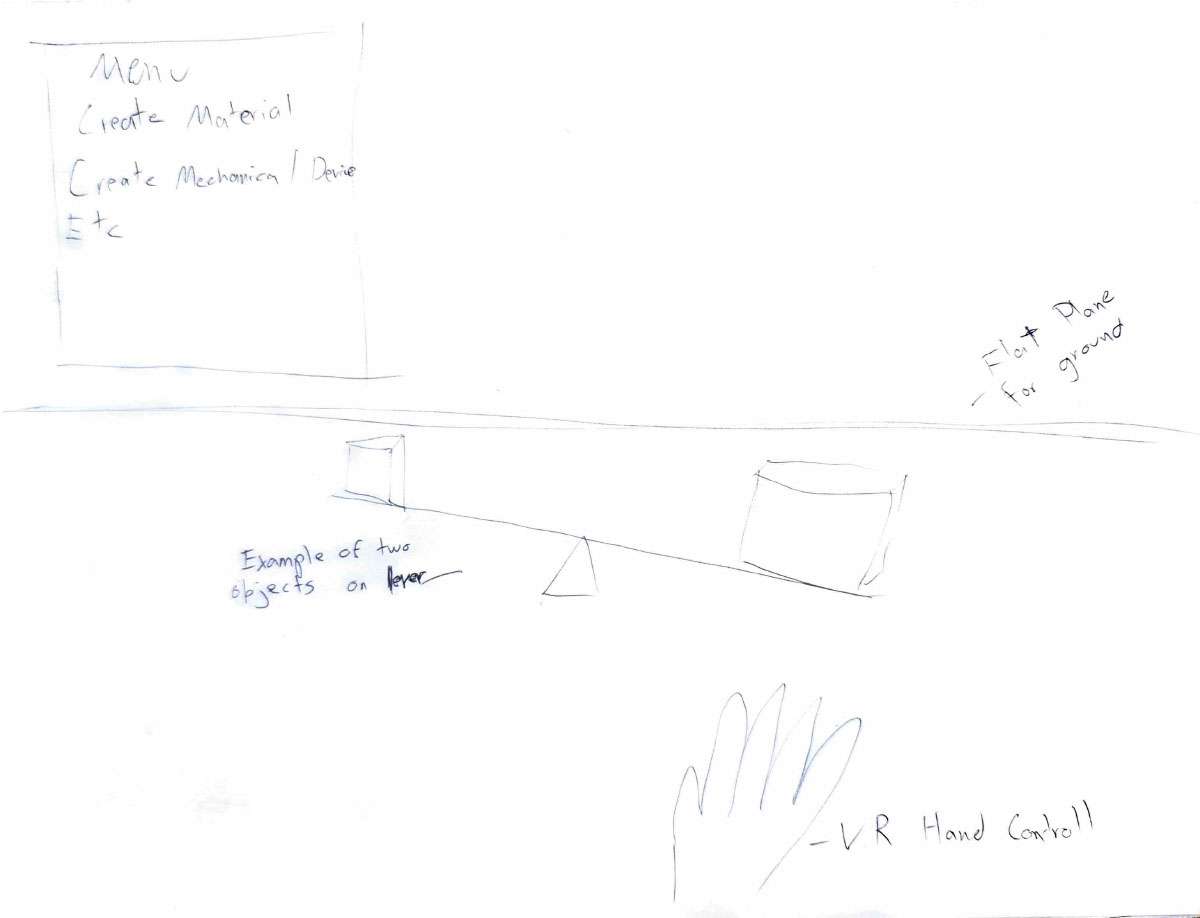
\includegraphics[width=\columnwidth]{HandDrawnMockup.jpeg}
  \caption{Hand-drawn concept sketch. From the learner's first-person view: a
  menu panel (create a material, create a mechanical device, and so on), two
  objects balanced on a lever over a fulcrum on a flat ground plane, and a
  tracked VR hand for direct grab-and-place interaction.}
  \label{fig:mockup}
\end{figure}

\begin{figure}[h]
  \centering
  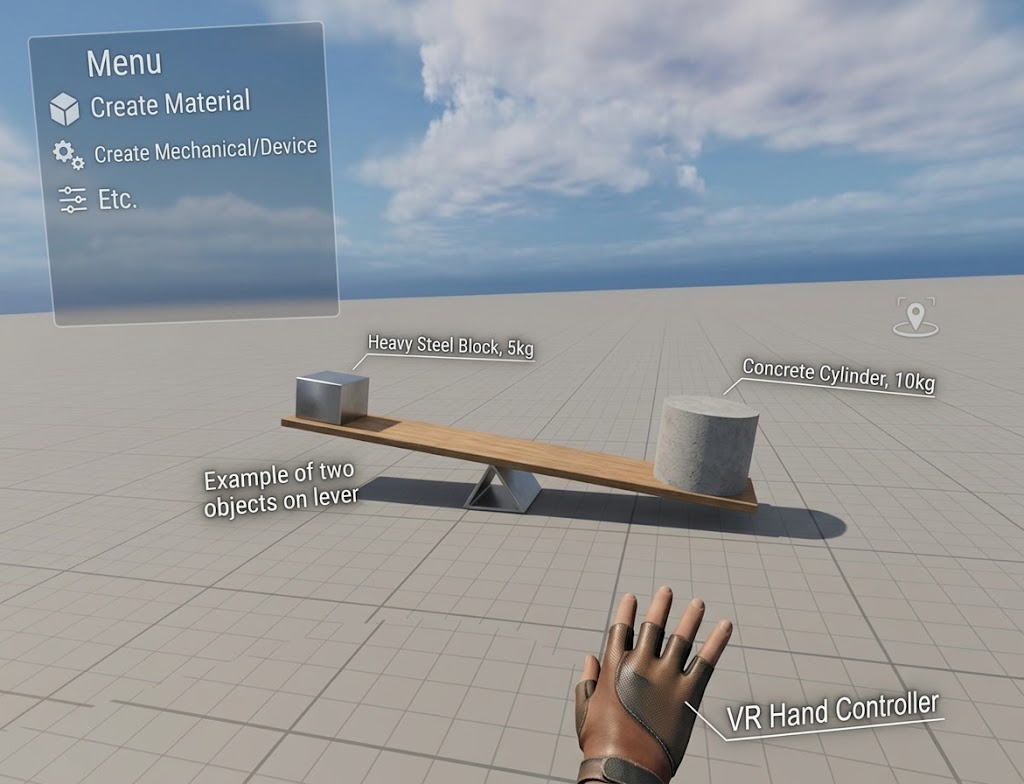
\includegraphics[width=\columnwidth]{GeminiEnhancedMockup.jpeg}
  \caption{AI-enhanced render of the same scene (generated with Google Gemini
  from the sketch in Figure~\ref{fig:mockup}). A labeled steel block and
  concrete cylinder rest on a lever, showing how the learner reads object
  properties and manipulates them by hand while the floating menu spawns new
  materials and mechanisms.}
  \label{fig:mockup-render}
\end{figure}

\section{Prototype Validation}
Before any human data is collected, the prototype must be shown to behave
correctly, and these system-level checks are a precondition for a meaningful
study. \textbf{Physics fidelity:} automated checks compare each scenario against
its closed-form prediction within a 5\% tolerance, for example that equal-mass
blocks show the correct relative volumes, objects float or sink by density, ramp
sliding follows the friction coefficient, and a lever balances at the computed
load position. \textbf{Pseudo-haptic behavior:} the cues must be monotonic, a
heavier object always feeling heavier and a more heavily loaded lever always
harder to move, with gain and lag mapping to mass and load in the intended
direction across the full range of materials and loads. \textbf{Performance:} the
scene must hold 72\,Hz on the Quest~2 so the cue is not confounded by dropped
frames. \textbf{Development workflow:} because agentic AI is our build method, we
report which parts of the implementation the coding agent produced through tool
use and iteration and where human correction was needed, drawn from a task log
kept from the first day of development. Passing these checks establishes that the
two builds differ only in the presence of the weight cue, which is what the study
in Section~\ref{sec:methodology} requires.

\section{Methodology and Study Design}
\label{sec:methodology}
Making a physical quantity \emph{felt} is only worthwhile if it changes what
learners understand, so beyond validating the system we run a small controlled
study with human participants.

\textbf{Research question.} Does a pseudo-haptic weight cue, added to direct
manipulation in VR, change how accurately learners predict outcomes that depend
on mass, density, and load, compared with the same manipulation without the cue?

\textbf{Design.} A within-subjects experiment with one independent variable, the
\emph{weight cue} (on vs.\ off), counterbalanced in order across participants. In
the cue-on build, control-to-display gain and visual lag track an object's mass
and the lever's load; the cue-off build uses plain grab-and-place with identical
visuals. Two matched scenario sets, A and B, are constructed so that no
participant sees the same scene twice, and set is counterbalanced against cue
condition. Held objects are made kinematic while grasped, the cue is applied to
the object's displayed position, and the object is handed back to the physics
engine on release, so that the simulation and the cue never fight each other.

\textbf{Dependent variables.} The primary measure is \emph{prediction accuracy}
on a short misconception test administered before and after each block. The six
items follow the style of the Force Concept
Inventory~\cite{hestenes1992force}: which of two equal-mass blocks is larger,
which floats, which slides farther down a ramp, where a lever balances, and two
transfer items using materials not present in the sandbox. Secondary measures
are: a two-alternative forced-choice heaviness judgment after each pair of blocks
(which felt heavier), serving as a manipulation check that the cue is perceived at
all; task completion time; and a five-item presence-and-comfort questionnaire
after each block.

\textbf{Procedure ($\approx$40 minutes).} Participants complete a pre-test, then a
short training scene, then block~1 (four scenes) followed by post-test~1, then
block~2 followed by post-test~2, and finally a brief interview on what felt
different between the two blocks. Cue condition and scenario set are assigned so
that order is counterbalanced across participants.

\textbf{Participants.} We recruit students who have not taken university physics,
drawn from non-physics courses, so that measurable misconceptions are present to
begin with. Because the design is within subjects, twelve participants are
sufficient for the scope of this class. Recruitment uses the standard class
data-collection form; this project is not intended for outside publication, so no
IRB submission is required. Were publication pursued later, an IRB with a faculty
principal investigator would be arranged before any recruitment began.

\textbf{Hypotheses.}
\begin{itemize}
  \item \textbf{H1:} the gain in prediction accuracy from pre-test to post-test is
        larger with the cue on than with the cue off.
  \item \textbf{H2:} heaviness judgments are above chance with the cue on and at
        chance with the cue off (the manipulation check).
  \item \textbf{H3:} reported presence is higher with the cue on.
\end{itemize}

\textbf{Analysis.} H1 is tested with a $2\times2$ repeated-measures ANOVA on
accuracy (cue $\times$ pre/post), with the interaction term as the effect of
interest. H2 is tested with a binomial test against chance for each condition. H3
is tested with a paired $t$-test on the presence score.

\section{Deliverables}
\label{sec:deliverables}
By \textbf{mid-November}:
\begin{itemize}
  \item A Unity 6 scene on Quest 2 with grab-and-place interaction for at least
        four materials, a working balance, a water tank, and a ramp, plus one
        mechanical device (a lever), all with pseudo-haptic weight and force
        modulation (gain and visual lag).
  \item Automated physics-fidelity checks comparing the simulation against
        closed-form predictions for density, buoyancy, friction, and the lever.
  \item In-scene logging of interactions and outcomes to file.
\end{itemize}
Toward the \textbf{early-December} presentation:
\begin{itemize}
  \item An expanded sandbox adding at least one more concept (for example a
        pulley or projectile launcher) built on the same interaction and physics
        framework, delivered as two builds (cue on and cue off) for the study.
  \item The within-subjects study of Section~\ref{sec:methodology} run with
        roughly twelve non-physics students, with the pre/post misconception
        test, heaviness manipulation check, and presence questionnaire analyzed
        as described.
  \item A recorded demonstration video walking through each concept on-device.
  \item The paper extending this proposal, documenting the design, the system and
        human evaluation, and a report on the agentic-AI development workflow used
        to build it, grounded in the day-one development log.
\end{itemize}
\textbf{Roles:} This is a solo project (group CS567\_SVEN). Sven Skoglund is
responsible for all work, including the Unity interaction and pseudo-haptics, the
physics-fidelity checks, the demonstration, and directing the agentic-AI
development workflow.

\section{Conclusion}
We are building a VR physics sandbox that turns abstract relationships, from
density and friction to the mechanics of levers and pulleys, into things a
learner can feel and test through direct, embodied manipulation. The application
is pure VR with no in-scene agent; agentic AI is the workflow used to build it.
The class should expect a working Quest 2 demonstration, automated checks that
the simulation matches the underlying physics, a within-subjects study of whether
the weight cue improves learners' physical predictions, and a report on how the
agentic-AI development process shaped the result.

\section*{Use of AI}
Generative AI (a large language model) was used to help locate candidate
peer-reviewed references and to critique the argument and grammar of drafts.
Google Gemini generated the enhanced mockup in Figure~\ref{fig:mockup-render}
from the author's hand-drawn sketch (Figure~\ref{fig:mockup}). The
implementation is planned as an agentic-AI development effort in which an AI
coding agent assists in writing and iterating on the Unity project under the
author's direction, and this will be documented in the final paper. All prose in
this proposal was reviewed and revised by the author, and every cited work was
read and verified by the author.

%% ---------------------------------------------------------------- references
\bibliographystyle{ACM-Reference-Format}
\bibliography{references}

\end{document}
